\mbox{}\\
\vspace{8cm}

This chapter is a reproduction of the following publication:

G. Fleres, N. Couto, L. Schuele, M. A. Chlebowicz, C. I. Mendes, L. W. M. van der Sluis, J. W. A. Rossen, A. W Friedrich, S. García-Cobos, Detection of a novel mcr-5.4 gene variant in hospital tap water by shotgun metagenomic sequencing, Journal of Antimicrobial Chemotherapy, Volume 74, Issue 12, December 2019, Pages 3626–3628, DOI: \url{https://doi.org/10.1093/jac/dkz363}

As referenced in section \ref{ssec:survaillance}, sequencing has become a common tool in surveillance and infection prevention, when combined with epidemiological data, have undoubtedly provided immeasurable insights regarding identification of potential sources of pathogenicity and transmission pathways. Shotgun metagenomic (SMg) approaches, just like in a clinical setting,  have been a growing interest to deliver relevant results without a priori knowledge of what to expect from a particular environmental sample. 

In this publication, second (see \ref{ssec:2nd_gen_seq}) and third (see \ref{ssec:3rd_gen_seq}) generation sequencing SMg has been applied to eight concentrated water samples collected the University Medical Center Groningen. In one of the samples, the novel detection of an \textit{mcr-5} gene, named \textit{mcr-5.4}, is reported. To the best of our knowledge, this is the first time that this gene, a mobile colistin resistance (\textit{mcr}) determinant, has been recovered from a hospital water environment, with analysis suggesting the order of \textit{Pseudomonadales} as the most probable host. 

My contribution to this publication included the bioinformatics analysis of the \textit{mcr-5.4} carrying sample thorough hybrid assembly using metaSPAdes. The resulting assembled contings were binned with the MaxBin2 tool and the bin having the sequence carrying the gene of interest was taxonomically characterised with Kraken2.


\cleardoublepage 

\begin{center}
\large
\textbf{Detection of a novel \textit{mcr-5.4} gene
variant in hospital tap water by
shotgun metagenomic sequencing}
\end{center}

Giuseppe Fleres$^1$, 
Natacha Couto$^1$, 
Leonard Schuele$^1$,
Monika A Chlebowicz$^1$,
Catarina I Mendes$^1$,
Luc W M van der Sluis$^2$, 
John W A Rossen$^1$, 
Alex W Friedrich$^1$, 
Silvia García-Cobos$^1$

$^1$ University of Groningen, University Medical Center Groningen, Department of Medical Microbiology, Groningen, The Netherlands;

$^2$ Center of Dentistry and Oral Hygiene, University
Medical Center Groningen, 9712 CP Groningen, The Netherlands

\section{Letter}

Sir,

Colistin is considered a last-resort antibiotic for treating serious infections caused by MDR Gram-negative bacteria. 
The efficacy of this antibiotic is challenged by the emergence and global spread of mobile colistin resistance (\textit{mcr}) determinants, which threaten human, animal and environmental health. 
The first mobile colistin resistance gene (\textit{mcr-1}) was reported in 2015 and since then up to eight different variants have been described \citep{wang_emergence_2018}. 
In 2017, Borowiak et al.\citep{borowiak_identification_2017} described a new transposon-associated phosphoethanolamine transferase mediating colistin resistance, named \textit{mcr-5}, in d-tartrate-fermenting \textit{Salmonella enterica} subsp. enterica serovar Paratyphi B isolated from poultry. 
The \textit{mcr-5.3} variant has been recently reported in \textit{Stenotrophomonas} spp. from sewage water \citep{li_co-occurrence_2019}.
Here we report for the first time (to the best of our knowledge) the detection of an \textit{mcr-5} gene in a hospital water environment using short-read metagenomic sequencing (SRMseq) and subsequent characterization using long-read metagenomic sequencing (LRMseq) to reveal its genetic environment.

In June 2017, eight tap-water samples (900 mL) were collected at the University Medical Center Groningen. 
Water samples were filtered (0.2 lm) and after DNA extraction (PowerWater DNA Extraction Kit, QIAGEN), SRMseq was performed on a MiSeq instrument (500 cycles) (Illumina). 
Antibiotic resistance genes were identified in the metagenome assemblies (CLC Genomics Workbench v10.1.1, QIAGEN) using ABRicate-0.7 (https://github.
com/tseemann/abricate) and applying the following thresholds:
.70\% identity and .80\% coverage. 
One sample contained an \textit{mcr}-type gene (5\% sequencing depth), with the nucleotide change 313C.T (amino acid change F105L) with respect to the original
\textit{mcr-5.1} gene, which was designated \textit{mcr-5.4} by NCBI (accession
no. MK965519). 
This sample was selected for LRMseq; the DNA libraries were prepared using the Rapid PCR Barcoding Kit (SQK-RPB004) from Oxford Nanopore Technologies (ONT) and
loaded into a FLO-MIN106 R9.4 flow cell. 
The run was performed on a MinION device (ONT) and it proceeded for 24 h. 
The data were basecalled using Albacore (https://github.com/rrwick/Basecallingcomparison) and further processed with Poretools \citep{loman_poretools_2014} and Porechop (https://github.com/rrwick/Porechop). 
Trimmed reads from SRMseq and LRMseq were used for hybrid-assembly analysis by
metaSPAdes-3.13.0 \citep{nurk_metaspades_2017}. 
After a BLAST search using the hybrid contig containing the \textit{mcr-5.4} gene, the plasmid pSE13-SA01718 (accession no. KY807921.1) was listed as one of the hits with the highest identity and we used it as a reference for genome comparison with the Artemis Comparison Tool (ACT) v1.0
\citep{carver_act_2005}. 
The \textit{mcr-5.4}-carrying contig from the hybrid assembly was annotated using PATRIC v3.5.27 \citep{wattam_improvements_2017}. 
Trimmed reads from SRMseq were used to investigate the bacterial composition by OneCodex \citep{minot_one_2015}. 
Finally, in order to predict the bacterial host of the \textit{mcr-5.4} gene, a contig-binning analysis of the hybrid-assembled metagenome was performed using MaxBin2 v2.2.4 (https://sourceforge.net/projects/maxbin2/), probability
threshold 0.9 and minimum contig length 1000 bp. 
The resulting bin containing the \textit{mcr-5.4} gene was selected for taxonomy classification using Kraken2 (https://github.com/DerrickWood/kraken2)
(minikraken2 DB v1).

\begin{figure*}[h!]
\centering
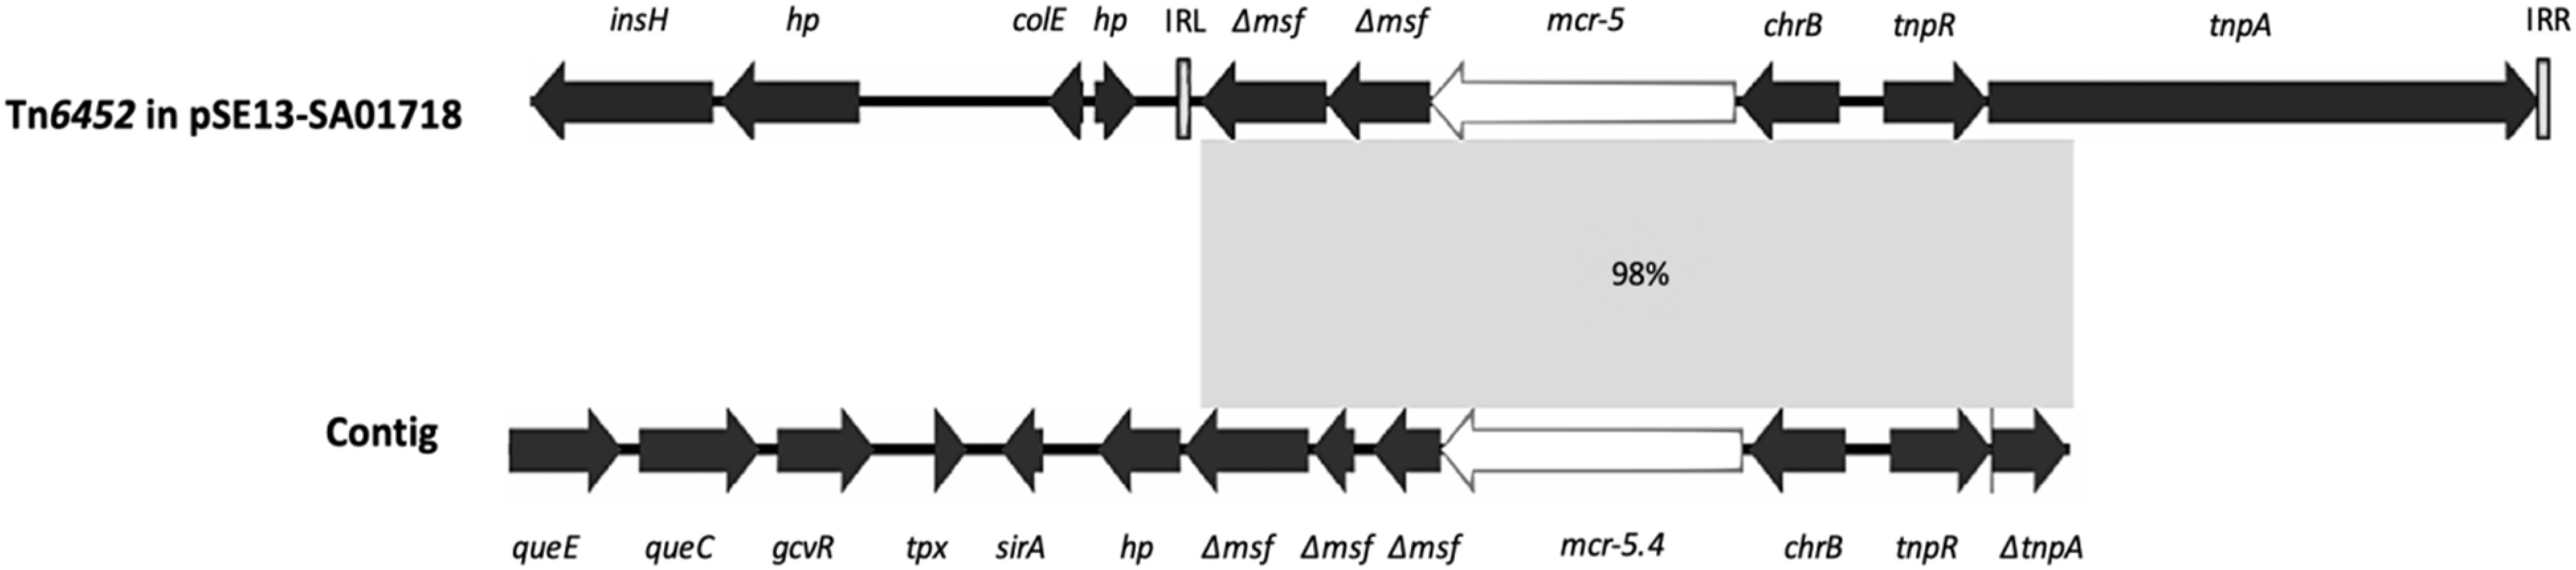
\includegraphics[width=\textwidth]{figures/chapter 3/dkz363f1.jpeg}
\caption{Comparative analysis of the genetic environment of \textit{mcr-5} between the reference plasmid pSE13-SA01718 (accession no. KY807921.1) and the annotated hybrid metagenome contig (accession no. MK965519). The contig carrying the \textit{mcr-5.4} gene consists of the following putative gene products: 7-carboxy-7-deazaguanine synthase (queE), 7-cyano-7-deazaguanine synthase (queC), glycine cleavage system transcriptional antiactivator GcvR (gcvR), thiol peroxidase (tpx), sulphurtransferase TusA family protein (sirA), hypothetical protein (hp), truncated MFS-type transporter ($\Delta$msf), lipid A phosphoethanolamine transferase (\textit{mcr-5.4}), ChrB domain protein (chrB), transposon resolvase (tnpR) and truncated transposon transposase ($\Delta$tnpA). Areas with 98\% identity between sequences are represented in light grey. Arrows indicate the position and direction of the genes. The transposon Tn6452 sequence in the reference plasmid pSE13-SA01718 is bounded by inverted repeats: IRL and IRR.}
\label{fig:chap3_figure1}
\end{figure*}


SRMseq showed the \textit{mcr-5.4} gene detected in a contig of 2113 bp flanked by two truncated protein-coding sequences (CDSs), encoding the ChrB domain protein (involved in chromate resistance) and the Major Facilitator Superfamily (MFS) transporter.
The hybrid-assembly analysis resulted in a contig of 8456 bp consisting of nine CDSs and four truncated CDSs (Figure \ref{fig:chap3_figure1}).
Comparative analysis of the genetic environment of the \textit{mcr-5} gene, between the annotated hybrid metagenome contig and the reference plasmid pSE13-SA01718, showed a region of 4670 bp with 98\% identity, corresponding to the backbone of the Tn6452 transposon (Figure \ref{fig:chap3_figure1}). 
We observed three truncated CDSs for the MFS-type transporter in our contig instead of two as previously described in the reference sequence pSE13-SA01718. 
These differences did not appear to be due to sequencing errors when we checked the sequence MK965519, (i) using pilon (https://github.com/broadinstitute/pilon) to correct for errors in short-read sequencing data and (ii) using CLC Genomic Workbench to update the hybrid contig by mapping both long and short reads against the hybrid contig.
We also observed a region of 3786 bp, with no identity either with the reference plasmid pSE13-SA01718 (Figure \ref{fig:chap3_figure1}) or with any other sequence in the GenBank database.

Species previously described to harbour an \textit{mcr-5} gene are \textit{Escherichia coli}, \textit{Pseudomonas aeruginosa}, \textit{Salmonella enterica}, \textit{Aeromonas hydrophila} and \textit{Cupriavidus gilardii}. 
The bacterial composition analysis of the water sample using SRMseq showed the presence of \textit{Pseudomonas} spp. (relative abundance: 0.004\%), \textit{Cupriavidus} spp. (relative abundance: 0.001\%) and \textit{Aeromonas} spp. (relative abundance: 0.0003\%). 
The binning analysis produced a bin positive for the \textit{mcr-5.4} gene consisting of 1336 contigs (genome size: 5 175 285 bp; genome completeness: 68.2\%). 
This bin was taxonomically classified as bacteria (70.73\%) and proteobacteria (64.90\%), and from this the most abundant class was \textit{Gammaproteobacteria} (37.20\%) (order \textit{Pseudomonadales}, 15.57\%), followed by \textit{Betaproteobacteria} (14.90\%) (order \textit{Burkholderiales}, 10.63\%).

Colistin resistance determinants (\textit{mcr}) have been rarely reported in water environments; \textit{mcr-1} has been detected in both hospital sewage and in environmental water streams and \textit{mcr-3} in environmental water \citep{zhao_incp_2017, tuo_prevalence_2018}.
To the best of our knowledge, this is the first-time description of an \textit{mcr-5} gene in an indoor and healthcare water environment. 
Despite the fact that the comparative analysis showed the hybrid contig covering a large region of Tn6452, neither the left inverted repeat (IRL) nor the right inverted repeat (IRR) have been found. 
In addition, the lack of the right transposon region does not allow us to search for other possible inverted repeats. 
Thus, it is not possible to conclude whether the described \textit{mcr-5.4} gene is transferable or not. 
Taxonomic analysis suggested the order of \textit{Pseudomonadales} as the most probable host of the \textit{mcr-5.4} gene in the water sample. 
Further studies are needed to determine the frequency of this gene in hospital water and other water environments and to evaluate the potential risks for patients and healthcare workers.

\section{Acknowledgements}

We would like to thank Erwin C. Raangs for technical assistance.

\section{Funding}

This project has received funding from the European Union’s Horizon
2020 research and innovation programme under the Marie SklodowskaCurie grant agreement 713660 (MSCA-COFUND-2015-DP ‘Pronkjewail’),
which includes in-kind contributions by commercial partners. None of
the commercial partners had any influence on interpretation of reviewed
data and conclusions drawn, or on drafting of the manuscript. This work
was partly supported by the INTERREG VA (202085)-funded project
EurHealth-1Health, part of a Dutch–German cross-border network supported by the European Commission, the Dutch Ministry of Health,
Welfare and Sport (VWS), the Ministry of Economy, Innovation,
Digitalization and Energy of the German Federal State of North RhineWestphalia and the German Federal State of Lower Saxony.

\section{Transparency declarations}

None to declare.